\subsection{Introduction \label{introduction}}

Modern science, engineering, and analysis workflows rely on computational tools for data processing, such as the foundational NumPy \cite{harris:nature20}, Pandas \cite{mckinney:scipy10}, Matplotlib \cite{hunter:cse07}, and Jupyter \cite{kluyver:ppap16} libraries for Python. Over the past few decades, different research areas and communities have built their own ``stacks'', i.e. layered sets of software tools that are combined to solve problems in a particular research area (see \cite{stancin:mipro19} for examples for big data, and \cite{briscoe:pcna00} for the idea of a layered stack). For instance, a Python geoscience stack might combine GDAL and Fiona for geoscience file-format access, Xarray \cite{hoyer:jors17} (itself built on NumPy) for multidimensional array processing, cartopy (built on PROJ and NumPy) for handling earth coordinates, Matplotlib for plotting, and Jupyter for user interaction and code execution. A Python financial analysis stack might combine Pandas for file reading and columnar data manipulation, Matplotlib for plotting, TA-Lib for financial mathematics functions, and Jupyter for user interaction and code execution.

Many of these stacks' components date back decades before Python became popular, capturing important functionality but inheriting technical complexity and limitations that may no longer apply. For instance, domain-specific visualization and user interface (UI) tools are often tied to a local desktop operating system and graphical user interface (GUI), limiting the stack to working with data and compute resources available locally, and making it difficult to share work with colleagues at other sites or using other operating systems. Older tools are often either inherently single threaded, with no support for distributed computation, or specifically focused on supercomputing systems rather than flexibly supporting the current diversity of computing platforms (such as GPUs and cloud computing). Software is of course infinitely malleable, and so any such limitations could be addressed \emph{in principle}, but in practice each domain-specific tool has a relatively narrow collection of users, contributors, and funding sources for that domain, limiting the scope of such development.

Could there be a better way? Yes! Today's Python ecosystem includes general data-processing tools that address tasks across all research areas, domains, and industries, with flexible tools for storing, reading, processing, plotting, analyzing, modeling, and exploring data of any kind. This paper introduces a specific collection of such tools called the Pandata stack. Like the ``modern data stack'' \cite{handy:dbtb20,jaipuria:substack22}, Pandata consists of tools that are engineered and tested to work well with each other to process very large datasets using distributed computation, with independently maintained components adding up to complete, end-to-end solutions for important workflows. Unlike the ``modern data stack'', the Pandata stack consists only of open-source tools and is also equally usable for small problems that fit onto a single laptop or local workstation, making it a solid basis for addressing data-centric problems of \emph{any} size for any domain.
% Also: https://www.fivetran.com/blog/what-is-the-modern-data-stack
% https://tanay.substack.com/p/understanding-the-modern-data-stack

The Pandata stack's Python libraries are:

\begin{itemize}
  \item\textbf{Domain independent:} Maintained, used, and tested by people from many different backgrounds
  \item\textbf{Efficient:} Run at machine-code speeds using vectorized data and compiled code
  \item\textbf{Scalable:} Run on anything from a single-core laptop to a thousand-node cluster
  \item\textbf{Cloud friendly:} Fully usable for local or remote compute using data on any file storage system
  \item\textbf{Multi-architecture:} Run on Mac/Windows/Linux systems, using CPUs or GPUs
  \item\textbf{Scriptable:} Fully support batch mode for parameter searches and unattended operation
  \item\textbf{Compositional:} Select which tools you need and put them together to solve your problem
  \item\textbf{Visualizable:} Support rendering even the largest datasets without conversion or approximation
  \item\textbf{Interactive:} Support fully interactive exploration, not just rendering static images or text files
  \item\textbf{Shareable:} Deployable as web apps for use by anyone anywhere
  \item\textbf{OSS:} Free, open, and ready for research or commercial use, without restrictive licensing
\end{itemize}

\begin{figure*}[t]
    \noindent\makebox[\textwidth][c]{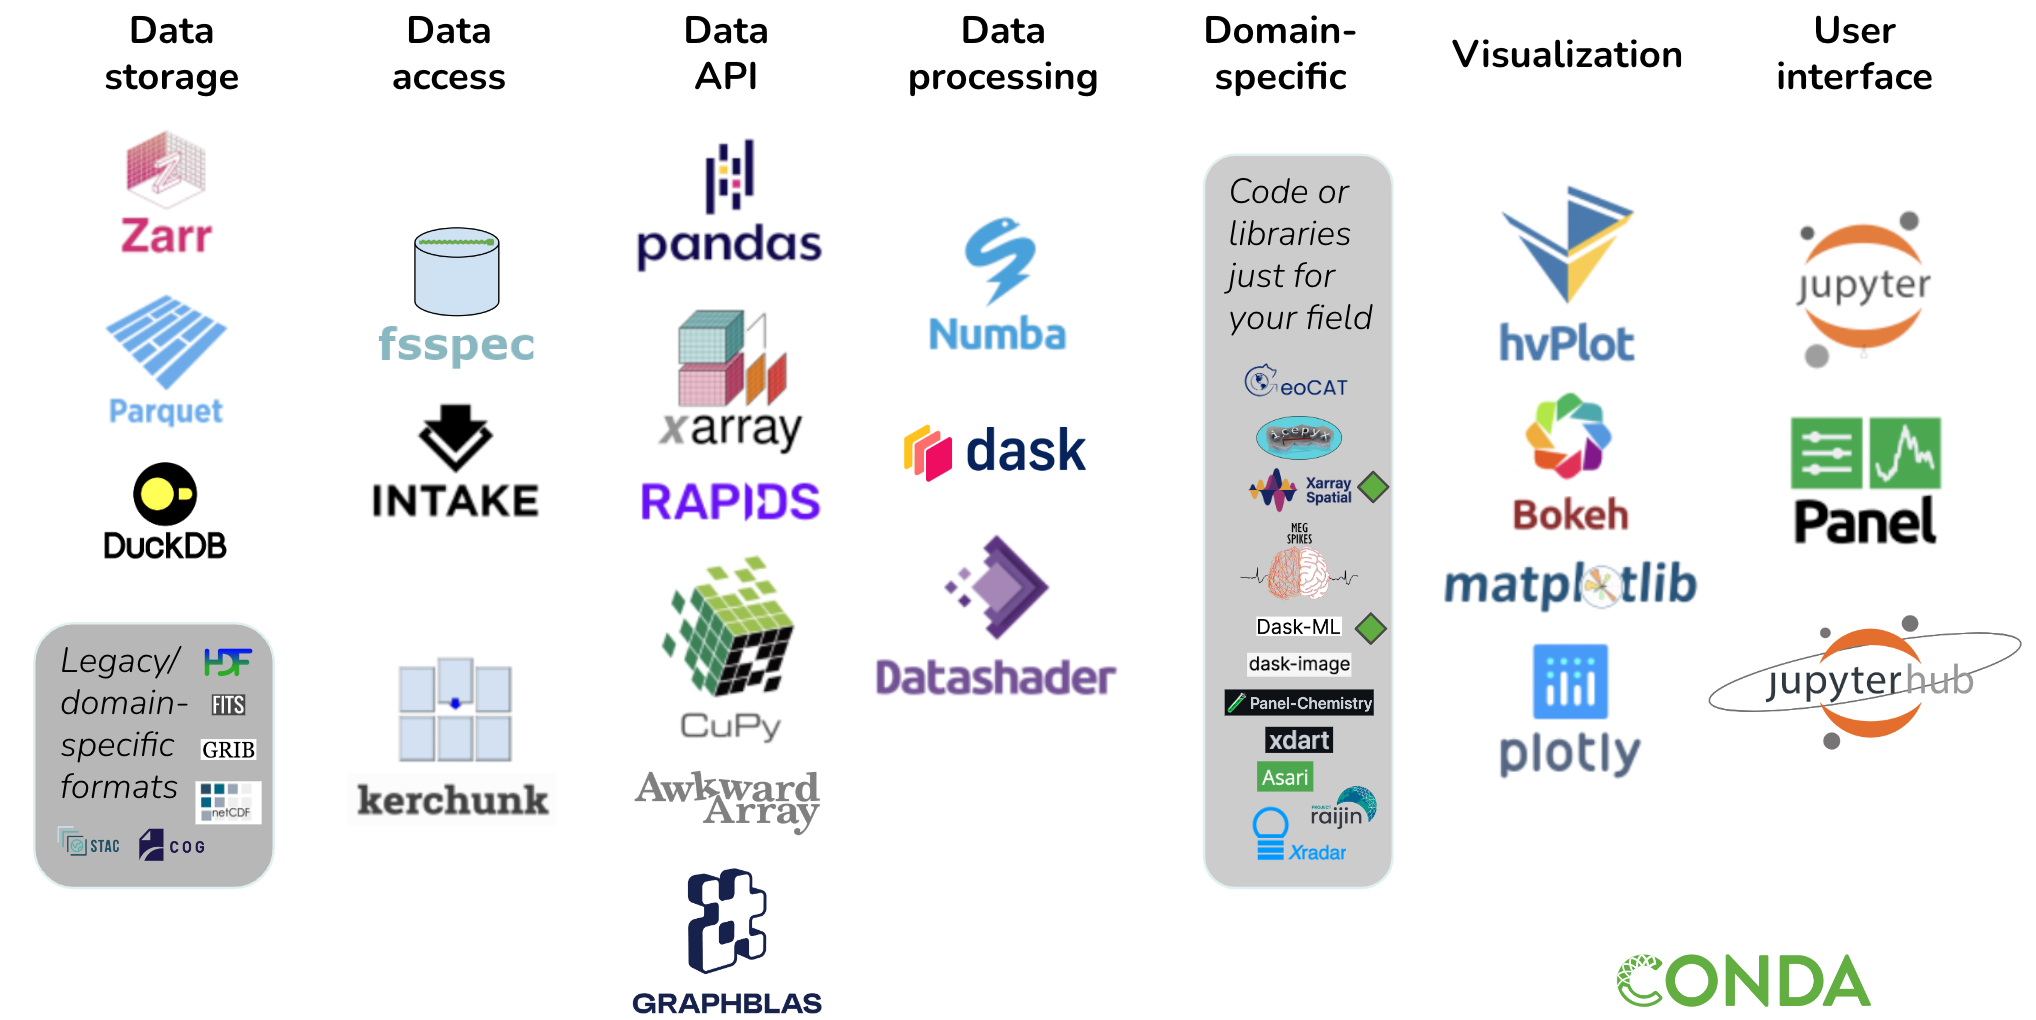
\includegraphics[width=\textwidth]{pandata.png}}
    \caption{Pandata: the scalable open-source analysis stack\label{pandata}.}
\end{figure*}
%%
Figure \ref{pandata} illustrates the Pandata stack, which includes the Parquet and Zarr file formats along with the fsspec, Kerchunk, Pandas, Xarray, RAPIDS, Dask, Numba, hvPlot, Panel, and Jupyter libraries. The tools are grouped into categories that will be described fully in later sections. Tools shown with a gray background are not part of Pandata itself but are illustrative of domain-specific code that builds on the Pandata stack to complete a solution for problems in a particular domain. We argue that Pandata libraries taken together as a group are a meaningful and well-tested base for general-purpose scientific computation across nearly all research areas and scientific domains. We will first look at the features that governed the selection of these particular libraries and that in many cases drive development priorities in the library itself. We will then describe the specific libraries involved and how they can be put together by users to solve computing tasks and how tool authors can build on them to support scientific computing in their own discipline.

\subsection{Design considerations}

Library authors have to choose between different designs and alternative technologies when deciding which features are implemented and how they are built.  Here we will unpack each of the above considerations driving the Pandata collection of libraries and examine how these libraries implement those principles.

\subsubsection{Domain independent}
Pandata tools are all built to be used in any scientific domain, without making design choices that constrain them to a narrow subfield or topic. At first it may seem that having all your tools be written specifically for your particular research area would be ideal, but we argue that it is neither desirable nor feasible to draw strict boundaries between active scientific research areas. Should you have to switch to an entirely different stack whenever you do collaborative work? Or if you want to do something novel, differing slightly from assumptions previously made in your research area? A deep, difficult-to-change stack that encodes a fixed and unnecessarily brittle model of your domain will make scientific progress difficult to achieve. Of course, not every aspect of research crosses multiple domains or challenges core assumptions, but using Pandata tools ensures that doing so will come at relatively little cost, because the same tools are valid across a very wide range of fields. Pandata tools can also draw from expertise, effort, and funding across all of science and analysis, rather than from a single narrow area.

\subsubsection{Efficient}
Because Python itself is a relatively slow, interpreted language, native Python code is often suitable only for smaller problems, limiting the audience for any tool that is built purely in Python with Python dependencies. To make efficient use of the computational resources available, libraries in the Pandata stack either wrap fast code written in compiled languages like Fortran and C, or they use a Python compiler like Numba \cite{lam:llvm15} or Cython \cite{behnel:cse11} to compile Python syntax into machine code that runs as fast as compiled C or Rust or Fortran. Custom domain-specific code building on Pandata can easily use a compiler like Numba as well, so that the overall workflows and pipelines are not limited by the speed of Python.

\subsubsection{Scalable}
Even compiled code is not sufficient to address the largest problems, which require more memory than is available on a single machine, or require long computation that is feasible only when split across many processors working simultaneously. To cover all these cases, Pandata tools support \emph{optional} distributed computation using Dask \cite{dask} on hundreds or thousands of processors, while also fully supporting a single laptop or workstation. That way there is no need to switch to a different stack when you hit a problem larger than your machine, or conversely when you want to work on small problems that do not need extensive infrastructure. Supporting distributed computation efficiently requires tooling support at every level, starting with chunked binary file formats like Parquet and Zarr that let each processor access data independently, and culminating in visualization tools like Datashader that can render plots in separate chunks on each processor and combine them for the final display. Note that Pandata includes libraries like Pandas and Matplotlib that are not necessarily scalable on their own, but become scalable when combined with other Pandata tools (with e.g. Dask providing scalable DataFrames built on Pandas DataFrames, and Matplotlib being scalable when used with Datashader).

\subsubsection{Cloud friendly}
The enormous datasets now available in many research areas are typically hosted in a remote data center and can be prohibitively expensive (in time and money) to download locally. If you only need a small part of the data, Pandata tools like Pandas support efficient remote access to the relevant chunks of each file without having to download it all locally first, using fsspec to provide uniform filesystem-like access for data on local disk, cloud storage, web servers, and many other locations. If the total size of the chunks that you need to access is still too high to download locally, Pandata tools also support remote computation, with the processing done on a remote cloud-computing server with a high-bandwidth connection to the data server and a user interface using a web browser whether compute is local or remote.  A typical scalable cloud-computing configuration for Pandata would be to have a remote JupyterHub system with Dask installed running on the cloud server close to the data. Users then contact the remote system from their local browser, initiating a remote session for computation and data access but with interactivity on the local machine using web-based controls and visuals. Using Datashader on the remote system provides server-side rendering so that only a rendered image of the data ever need be transferred across low-bandwidth connections, providing interactive local visualization without having to transfer large datasets. Pandata tools thus support either efficient access to remote datasets for local computation, or efficient fully remote computing with a local user interface, to make good use of cloud storage or compute resources. Note that ``cloud friendly'' is not the same as the term ``cloud native'' as used in the Modern Data Stack; Pandata tools fully support cloud usage but are equally at home on a local machine, and have no requirement for cloud resources, containers, microservices, or other architectures typical of cloud-native approaches.

\subsubsection{Multi-architecture}
Because researchers typically use Windows or Mac systems locally, while cloud servers typically run Linux, research code needs to be independent of the operating system for it to be equally well supported on local and remote systems. A software stack tied to a particular OS not only shuts out users who are not on that OS, it often implicitly favors either cloud or local usage for that stack, further reducing the community size and range of problems that can be addressed by a particular stack. Pandata tools are all either fully OS independent or support Linux (Intel or ARM), Mac (Intel or M1/M2), and Windows. Similarly, some problems can be addressed orders of magnitude faster on a general-purpose graphics processing unit (GPU) than on a conventional CPU, yet many researchers do not have access to GPUs or are working on problems unsuited for them, making it essential that a general-purpose software stack support both GPU and CPU usage as appropriate. The Pandata stack includes GPU-based equivalents for much of the functionality available on CPUs.

\subsubsection{Scriptable}
Many of the scientific tools that are common in particular domains (especially commercial tools provided alongside hardware used in that domain) require a GUI. GUI tools can be convenient for exploration, but without an accompanying non-GUI interface it is difficult to capture a reproducible set of steps for publication and dissemination. Additionally, GUIs often funnel users into a few well-supported operations without providing the level of configurability and customization needed to execute less common workflows, long-running jobs, or large parameter searches. Pandata tools that offer a GUI interface never require a local desktop, graphical display, or live interaction, making them fully suitable as a basis for reproducible, large-scale, and long-running research.

\subsubsection{Compositional}
When approaching a particular task, a researcher can either choose a monolithic tool that addresses all aspects of the task, or they can combine lower-level tools that together accomplish the task. Monolithic tools are attractive when they fully cover a specific use case, but given the dynamic nature of research, it is unreasonable to expect a monolithic tool to cover all the requirements of a particular research area, let alone across different areas of research. Accordingly, Pandata tools are all compositional, intended for independent use or in combination to solve specific problems. Where appropriate, each library has been adapted to work well with components from the other Pandata libraries, allowing a researcher to mix and match and combine projects in novel ways to reach their goals. Pandata projects also take part in larger efforts to improve compositionality and interoperability like \texttt{numpy.org/neps} and \texttt{scientific-python.org/specs} and by implementing existing APIs that allow a Dask dataframe to be a drop-in replacement for a Pandas dataframe, let hvPlot be a drop-in replacement for Pandas plotting, or allow a Panel app to display ipywidgets (or vice versa). Of course, compositional approaches can take more initial user effort and expertise than an out-of-the box monolithic approach. To address well-established complex tasks, a domain-specific monolithic tool can be built out of Pandata tools, while other tasks that need to remain flexible can be built compositionally as needed for that task.

\subsubsection{Visualizable}
For computing tasks that operate in the background without any visual output, it is easy to ensure that they are scriptable and cloud friendly. However, doing good science requires understanding each of the processing steps in complete detail, and if there are any unobservable black boxes in your workflows, that is surely where bugs will hide. To make sure that the work is being done correctly, it is crucial to be able to represent each of the computing steps involved in a way that a human can easily grasp what is happening, with a minimum of extra effort that discourages exploration. Often, a remote computing job will export data that is then subsampled and downloaded locally for analysis, but any step that adds friction and covers up the raw data makes it more likely that important issues and insights will be missed. Accordingly, the HoloViz tools included in the Pandata stack are designed to make the full set of data available at any point in the computation, by supporting efficient in-place interactive visualization of even distributed or GPU-based data of any size using Datashader and hvPlot, assembled from separately computed chunks for display on any device.

\subsubsection{Interactive}
Supporting unattended batch-mode computation is important for doing comprehensive parameter evaluation, but batch runs tend to keep research focused on specific well-trodden paths, changing only a few options at any one time and thus limiting the search space that gets explored for a model or dataset. Using only a batch approach makes it easy to miss important opportunities or to fail to understand major limitations, by simply re-running the same code paths ``blind'' every time. Pandata tools like hvPlot and Panel running in Jupyter make it easy even for remote cloud workflows to have interactive widgets and controls in a web browser, to more easily explore parameter combinations with immediate feedback to help understand how the system behaves.

\subsubsection{Shareable}
Creating easy interactive visualizations is great, but if they are limited to your own desktop or installation, the impact of your ideas and approaches will be limited. With enough HTML/JavaScript/CSS web-technology experience, any computation can be wrapped up as an interactive website, but many scientists lack front-end web-development skills. The Panel tool in Pandata makes it simple to convert any Jupyter notebook into a web app that can be shared with collaborators or the public to disseminate the results of a project. Panel apps can be shared as static JavaScript-based HTML files (for small datasets), WASM-based HTML files (running Python in the browser), or via a live Python server (for the largest computations and datasets). (Also see ``Environments and reproducibility'' below for other aspects of ensuring that your work is shareable.)

\subsubsection{OSS}
For software to be fully accessible across years, labs, collaborators, and research problems it is crucial that there be no licensing restrictions that prevent it from being used across the entire discipline and on all relevant hardware and software platforms. Pandata tools are all permissively licensed so that they are freely usable in academia, industry, government, and by private individuals, easily scaled up to the largest problems or in new contexts without having to obtain permission or pay additional fees. Beyond the licensing, it is also crucial that the underlying source code is accessible, so that every processing step involved can be examined and justified. That way, if the research hits any fundamental limitations, it is always possible (though not always easy!) to extend or adapt the software for the new requirements. The OSS developer community is also typically accessible through issues and online forums, so that even though the software is not officially ``supported'' in the sense of commercial software, it is often easier to discuss details of the software's internal operations with the maintainers than with commercial software where developers are inaccessible.

\subsection{The Pandata stack}

The above considerations determined which libraries are considered to be a part of the Pandata stack. As illustrated in Figure \ref{pandata}, the stack consists of options for each of the major steps in a data-processing task. A finance task might involve files from efficient Parquet-format columnar data storage, accessed from Amazon S3 storage using fsspec file readers, into a Pandas data API, for data processing using Pandas calls plus some custom Numba-optimized analysis code, visualized using an interactive Bokeh plot returned from hvPlot, using Jupyter as a UI (figure \ref{pandata-finance}). When moving to larger financial datasets or more complex analysis and processing, a Dask dataframe can be substituted for the Pandas dataframe, while keeping the rest of the tools the same, thus supporting distributed computation without requiring it.
%%
\begin{figure*}[h]
    \noindent\makebox[\textwidth][c]{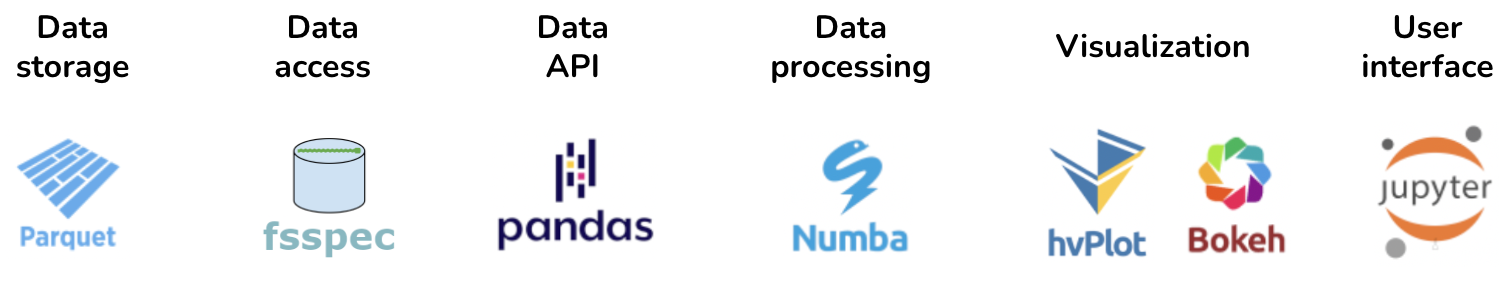
\includegraphics[width=0.987\textwidth]{pandata-finance.png}\hfill\hbox{}}
    \caption{Pandata stack applied to a finance problem\label{pandata-finance}}
\end{figure*}
%%
Similarly, a geoscience task typical for the Pangeo community might involve files stored in cloud-friendly Zarr multidimensional array storage, accessed using fsspec based on a specification in an Intake data catalog, into a lazy Dask-based xarray multidimensional data structure, with raster processing done by the Xarray-spatial library (not part of Pandata since it is domain specific, but built on the Pandata stack and using otherwise similar principles), with visualization using xarray's interface to Matplotlib for Dask data structures, and with computation and a UI provided by JupyterHub running in the cloud and providing access to Jupyter (figure \ref{pandata-geoscience}).

As you can see from these examples, any particular problem solved using the Pandata stack can involve completely different underlying libraries, and because each of the Pandata libraries are designed to interoperate freely, users can select the appropriate library or libraries for their needs at each stage. We'll now look into each of the stages in a bit more detail to explain the options available to a researcher using Pandata tools to solve their particular research problems.


\subsubsection{Data storage}

Pandata tools are designed for working with data, whether it comes from a file on disk, a hardware device, remote cloud storage, or a database query. Many existing scientific file formats were designed before cloud computing and are \emph{terrible} choices for efficient distributed computation. The ubiquitous comma-separated-value CSV columnar file format, for instance, can be orders of magnitude larger and slower than Parquet (\texttt{github.com/holoviz/datashader/issues/129}). CSV and other legacy formats also often require serial access to the whole file to reach any value in it, thereby preventing parallel reads by processors working on different parts of the task. Even relatively efficient older binary formats are typically not ``chunked'' in a way that makes it simple to access the data needed by any particular run or any particular processor in a large compute job.

Pandata tools can provide very efficient, scalable, end-to-end computations only if the data itself is stored in an efficient, chunk-addressable way. Parquet is a suitable well-supported chunked columnar format (for data arranged in rows consisting of differently typed columns), while zarr is a suitable chunked multidimensional array format (for $n$-dimensional arrays of typed values indexed by row, column, and other dimensions). DuckDB is a relatively new addition to Pandata that makes an underlying file type like CSV or Parquet act like a queryable database, which can be very efficient when accessing small parts or aggregations of large datasets, so other Pandata tools are starting to add support for working with DuckDB as well.

What if you need to access very large collections of data \emph{not} already stored in an efficient chunked format like Parquet or Zarr? Thanks to kerchunk (see ``Data access'' below), it is possible to scan such files to record the locations of each chunk of data stored in them, and from then on act as if the underlying file is in Zarr (or potentially Parquet) format. In this way, the Pandata stack can support access to a wide array of legacy binary file formats such as HDF/NetCDF, GRIB, FITS, and GeoTIFF, which with the appropriate Kerchunk driver can now support efficient scalable computation without servers having to maintain multiple copies of the underlying data.

\subsubsection{Data access}

Once you have data in a suitable supported file format, it needs to be located somewhere that your Python code can access it. The nearly invisible but powerful fsspec library provides flexible and efficient access to files wherever they might be located, whether that is on your local hard drive, on an FTP file server, on cloud storage like S3, on a website, in a zip file, or in any number of other possible locations. fsspec is now integrated into Pandas and Xarray, transparently providing access from within those libraries (below). As mentioned above, Kerchunk can optionally be used for data access to make an older file format be efficiently addressable for Pandata usage, once there are indexing plugins available for that particular (usually domain-specific) format. Kerchunk and fsspec are also supported by the Intake data-catalog system, which allows a research group or community to capture metadata about collections of datasets so that they can be accessed conveniently without having research code tied to the location or file type of the underlying data.

\subsubsection{Data API}

At a Python level, most users actually start here, by selecting an appropriate data application programming interface (API) for their work. Python libraries provide many possible APIs that are suitable for different types of data. Pandas (for columnar data) and Xarray (for multidimensional data) are both supported throughout the Pandata stack, with or without Dask (see below) to handle distributed and out-of-core computation. Pandata's other options provide access to other data structures (ragged arrays, for Awkward, and graphs/networks, for GraphBLAS) and/or other computational hardware (RAPIDS and CuPy for GPU architectures), with extensive (but not yet fully complete) support throughout the Pandata stack. Users or domain-specific library authors will typically pick one or more of these data APIs to cover the types of data being used in their domain or their specific problem, and then provide a path to the data to access it using the underlying data-access tools using the data formats and storage available.

\subsubsection{Data processing}

Once the data is accessible in Python using a data API, the actual computation can begin. Data processing covers many possible computations, but we will consider three main categories: (1) domain-general operations provided by the data API library directly, (2) small custom-compiled loops for arbitrary domain-specific computations at scale, and (3) separate domain-specific or other custom libraries. (1) First, each data API provides a wide variety of inbuilt data-processing routines for selecting, aggregating, and summarizing the data being accessed. For many data-processing workflows, such transformations are sufficient to complete the task, when combined with the rest of the Pandata stack, and using them preserves all the Pangeo qualities like scalability and easy visualization. (2) Second, sometimes the domain-specific code can be isolated to a few small loops with explicit numeric or string computations, now that Pandata covers so many of the other tasks. In such cases, these loops can easily be implemented in a notebook or script using the general-purpose Numba library along with Dask for optional scalability, again providing all of the benefits of Pandata without significant effort.

(3) The third category of computations typically requires leaving the Pandata stack, bringing in domain-specific libraries from the Python ecosystem that focus on the particular models and computations needed in a given domain. In some cases, you can find domain-specific libraries already designed to work well with the Pandata tools like Dask and Xarray, e.g.\ xarray-spatial (geoscience), dask-image (image processing), dask-ml (machine learning), icepyx (satellite data), panel-chemistry (chemistry), xdart (x-ray analysis), asari (metabolomics), and megspikes (brain imaging). Using a Pandata-compatible domain-specific tool helps ensure that all of the above properties like being scalable, visualizable, and cloud-friendly are maintained. However, in other cases there will be libraries available, but using them will introduce a bottleneck: not being scalable with Dask, not being compiled for efficient operation, not being vectorized to work with large datasets, being tied to a local GUI or local filesystem access, etc. In those cases, you can either try to ensure that the bottleneck only applies to infrequent usage patterns, or you can invest what may require substantial effort to rewrite the domain-specific libraries to work well with a Pandata approach. Rebuilding a particular domain's tools to be fully integrated with the Pandata stack takes time, requiring ambitious projects like building your simulator or analysis tool on top of Dask and Xarray or Pandas and ensuring that fully visualizable distributed objects are available for all stages of a workflow. Still, the focus of such efforts can be solely on the aspects specific to a particular research domain, and they can simply inherit all the capabilities of the Pandata stack (now and into the future) for what the Pandata stack covers.

%%
\begin{figure*}[h]
    \noindent\makebox[\textwidth][c]{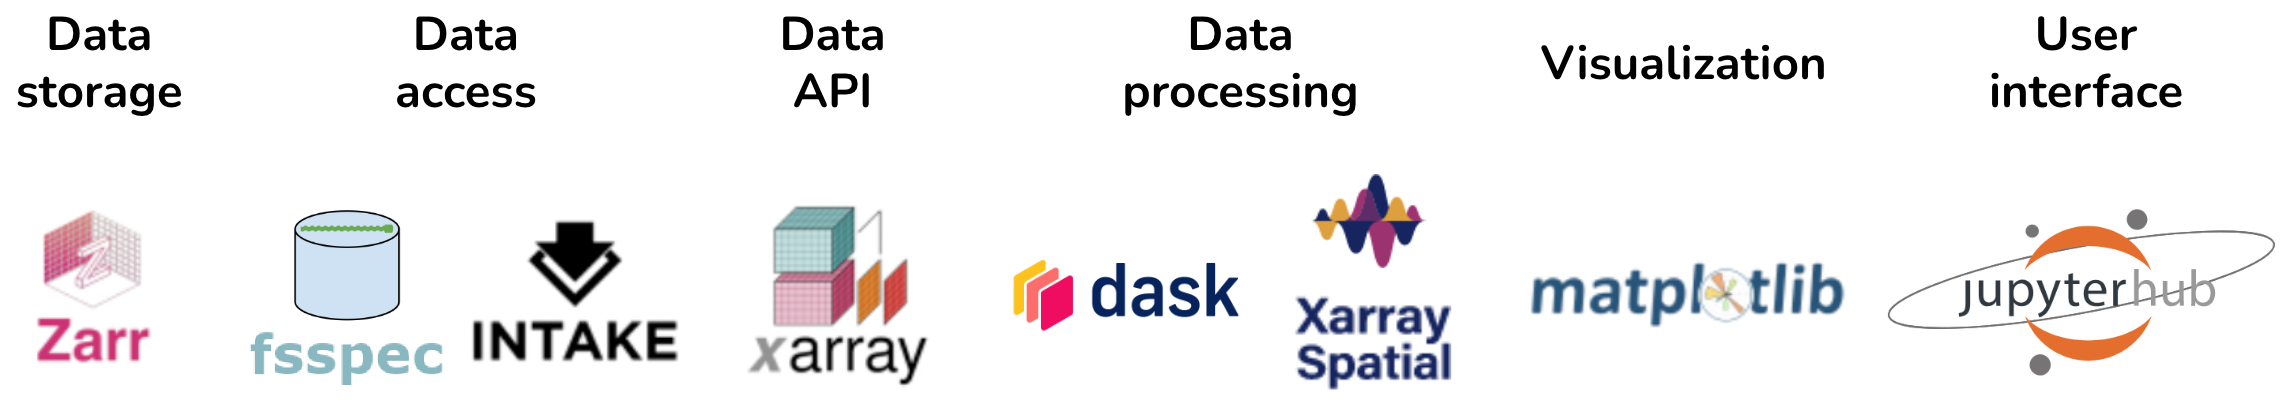
\includegraphics[width=\textwidth]{pandata-geoscience.png}}
    \caption{Pandata stack applied to a geoscience problem\label{pandata-geoscience}}
\end{figure*}
%%
\subsubsection{Visualization}

Each step in the complete data-processing pipeline pipeline from raw data to results requires human understanding and validation, often most effectively achieved using visualization tools. Most Python visualization tools (see \texttt{pyviz.org} for a complete list) have limitations that prevent them from being suitable for the Pandata stack. Many of them are limited to relatively small amounts of data, lack support for the various Pandata data APIs, lack support for multidimensional arrays or unstructured grids for the fields that need those, or are tied to a desktop OS or GUI. All Pandata tools support basic static-image visualization using Matplotlib, and most also support fully interactive Bokeh- or Plotly-based plotting via hvPlot \cite{rudiger:hvplot}. hvPlot supports the native \texttt{.plot} visualization calls provided by the data APIs, while adding support for efficient server-side distributed rendering using Datashader so that even the largest datasets can be visualized without subsampling or copying the data. Datashader can also be used by itself as a general-purpose scalable server-side rasterizer, turning data of any supported type (point, line, region, polygon, raster, etc.) into a regular grid of values suitable for further processing and combination with other data.

\subsubsection{User Interface (UI)}

The Jupyter Notebook is a now-ubiquitous domain-independent user interface for working with Python code, and all Pandata tools are fully usable from within Jupyter. Beyond just executing cells full of code, the Panel library in Pandata makes it simple to add interactivity to each Jupyter cell, using a widget to provide control over workflow parameters, and allowing tabular or graphical outputs to be arranged into dashboards or small applications that fit into a cell. Panel also lets users designate certain cells as being ``servable'' if the notebook code is deployed as a separate, standalone application with a UI independent of Jupyter. Panel thus supports the ``interactive'' and ``shareable'' qualities of the Pandata stack, ensuring that your work can have impact on others.

Jupyter focuses on a single researcher or user, but many Pandata-based projects involve collaborations among multiple team members and multiple institutions. Such projects typically use JupyterHub to provide a shared computing environment with the Pandata tools already installed and ready to run. Pandata-based projects often use Nebari (a declarative specification for infrastructure) to simplify configuring JupyterHub, Dask, and associated authentication on cloud servers.

\subsubsection{Environments and reproducibility}

A final category of tools underlying all the rest shown in figure \ref{pandata} centers on how these libraries are packaged and put together into Python environments for solving any particular problem. Many different options are available for Python package and environment management, but Pandata tools are typically used with the conda package and environment manager, because it tracks binary dependencies between libraries, including the underlying C and Fortran code that is involved in the domain-specific libraries needed for any particular Pandata workflow. For a specific workflow, once the list of packages needed in the environment has been finalized, the anaconda-project tool (now being developed in a more general form as conda-project) allows the precise versions involved to be locked on every supported platform, achieving cross-platform reproducibility for a Pandata-based project (see
\cite{bednar:anaconda22} for details).


\subsection{Examples}

To help users understand how these tools fit together, a variety of example workflows based on Pandata tools can be found online. The website \texttt{examples.holoviz.org} includes research topics in different domains, with Pandata tools featured prominently in most of them and particularly in the Attractors, Census, Ship Traffic, and Landsat examples. The \texttt{holoviz.org} site has a tutorial that brings in many of the Pandata packages to solve an example research problem. The Pangeo Project Gallery at \texttt{pangeo.io} and Project Pythia at \texttt{projectpythia.org} both include detailed examples in the specific area of climate science. Each Pandata package also has its own documentation and website illustrating what it can do, often in combination with other Pandata tools, such as the Dask examples at \texttt{stories.dask.org}.

\subsection{History and background}

The Pandata libraries individually address important domain-independent problems for scientific research, engineering, and data analysis. As argued above, together they form a coherent and powerful basis for scientific computing in any discipline. Given that each tool has its own developers, separate management structures, and separate communities, how did it happen that together the tools add up to such a coherent approach? To understand this process, it is necessary to dive into the history of some of these projects and the connections between them.

First, many of the Pandata projects were either originally launched at Anaconda, Inc., or they were adapted by people who were at Anaconda at the time to work well with the other projects. Anaconda's consulting division (led by the author Bednar) and open-source tooling division (with most projects led by the author Durant) have worked with a wide variety of government agencies, private foundations, universities, and companies doing numerical computation and research. Each project is designed to address pain points being experienced by those collaborators, and the Anaconda staff involved help the projects work together to add up to complete solutions. Each new consulting project also extensively tests and validates each library both alone and in combination with the others, ensuring that these particular packages add up to complete solutions for each domain in which they are applied.

Specifically, the fastparquet, fsspec, kerchunk, intake, numba, dask, datashader, bokeh, hvplot, panel, and conda projects were all created by developers working at Anaconda at the time, with funding from a very wide range of external grants and contracts but with Anaconda playing a central role in developing them and ensuring interoperability between them. These Anaconda-based developers have also contributed extensively to the other projects listed, such as xarray, pandas, awkward-array, graphblas, zarr, and jupyter. Anaconda as a company does not (and cannot!) control the overall set of projects involved, because each has their own contributors, governance structure, and stakeholders. But having a large collection of scientific software developers working at Anaconda on this wide range of projects exercising the code in many different research fields and domains has led naturally to the emergence of Pandata, to which this paper is only now assigning a name and describing the underlying principles guiding this work.

Out of the many external projects that Anaconda developers have been involved in, there is one that deserves a special mention because of how it catalyzed the collection of Pandata tools: Pangeo \cite{odaka:tthpc20}. The \texttt{pangeo.io} project is a climate-science initiative based on bringing modern distributed cloud computing approaches to bear on large-scale modeling and analysis of the Earth's climate. Many of the Pandata tools are also Pangeo tools, and in fact the main distinction between Pandata and Pangeo is simply that Pangeo is domain specific, while Pandata is largely the same stack of tools as Pangeo but explicitly not being tied to any specific research domain (hence the name ``Pandata'', with Pangeo-style tooling but for any field using data, not just geoscience). Across numerous grants, contracts, and projects, Pangeo's researchers have improved each of the various tools in the Pandata stack and demonstrated how they can be put together to solve very challenging research problems, cost-effectively processing petabytes of climate and remote sensing data in a way enabled by Pandata tools like Dask and JupyterHub. This paper is an effort to publicize that the underlying tools are in fact fully domain general and applicable to \emph{all} of science, with different data API and file format choices but largely the same tools used to cover general data-processing needs that span all research areas. Why start from scratch, when you can build on this battle-hardened, extensively validated set of general-purpose tools addressing much of what you need in any project?

\subsection{Alternatives to Pandata}

The libraries in Pandata are of course not the only alternatives available in Python; each library individually has alternatives that have their own strengths and advantages. However, the alternative libraries have not (yet?) been integrated with Pandata tools, making it much more difficult to apply them to a Pandata-based project. For instance, Ray \cite{moritz:arxiv18} is an alternative approach to distributed computation that is not supported by these tools, and so if a project uses Ray to manage distributed computation, then they cannot (currently) easily select hvPlot for visualization without first converting the data structures into something hvPlot understands. Similarly, Vaex \cite{breddels:aaa18} and Polars \cite{ritche:polars} offer alternatives to the Pandas/Dask columnar dataframes supported in Pandata, and projects based on those data APIs will not (yet!) easily be able to use Pandata tools for visualization and user interfaces. There are also now alternative tools for server-side rendering of large datasets that in Pandata are handled by Datashader, such as VegaFusion for Vega and Altair, but those are not fully integrated with the other Pandata libraries like Dask and Numba.
%  ray does have an explicit integration with dask; not clear how much it is in use

There are also full alternative stacks to consider, such as tools like Hadoop \cite{white:hadoop15} and Spark \cite{zaharia:cacm16} from the Apache Foundation. Most Apache tools rely on the Java Virtual Machine (JVM) that provides OS-independent computation but requires a heavyweight runtime compared to the Pandata tools, making it awkward to combine most Apache tools with Pandata tools. Pandata already offers flexible support for distributed computation without the JVM overhead, making ``big data'' tools like Hadoop and Spark unnecessary for Pandata applications. Pandata does rely on the low-level Apache Parquet and Arrow projects, which have non-JVM implementations that fit well into the Pandata stack.

\subsection{Future work}
This paper is the first to describe Pandata as an entity or collection of tools. The specific tools we selected are those that in the opinion of the authors are well integrated with the other tools and provide a ``mix and match'' approach to putting together libraries to implement a particular analysis workflow. There is not currently any entity besides these authors and this paper that defines what Pandata is, which libraries are included, and what process to follow for a library to be included or excluded from Pandata. As Pandata evolves, it will be important to formalize some of these processes, similar to how the Pangeo organization and the HoloViz organization (of which hvPlot and Panel are a part) have been constituted with a independent steering committee and governance policies. Future Pandata directions and development can be tracked at \texttt{github.com/panstacks/pandata}, where people interested in Pandata can raise issues and discuss options and alternatives. In the meantime, Pandata is just a concept and an explanation for the work of hundreds of people working mostly independently but with key connections that make these independent projects come together into a coherent stack for performing scientific research.

Other relevant areas that need work include the development of domain-general reusable tools for capturing the metadata, conventions, consistent units, etc. needed in each domain, such as the \texttt{cfconventions.org} conventions for climate science. Furthermore, improved tools for collaboration are needed, such as implementing parts of the JupyterHub roadmap (\texttt{jupyterhub.readthedocs.io/en/stable/ contributing/roadmap.html}). Lastly, better documentation and workflow demonstrations of the Pandata stack are required to facilitate easier onboarding, provide comprehensive usage guidelines, and showcase the full potential of Pandata in solving diverse scientific problems.


\subsection{Conclusion}

The Pandata stack is ready to use today, as an extensive basis for scientific computing in any research area and across many different communities. There are alternatives for each of the components of the Pandata stack, but the advantage of having this very wide array of functionality that works well together is that researchers in any particular domain can just get on with their actual work in that domain, freed from having to reimplement basic data handling in all its forms and freed from the limitations of legacy domain-specific stacks. Everything involved is open source, so feel free to use any of these tools in any combination to solve any problems that you have!

\subsection{Acknowledgements}

Thanks to Christian Capdeville, Deepak Cherian, Andrew Donoho, Kodie Dower, Tetsuo Koyama, Dillon Niederhut, Dharhas Pothina, Demetris Roumis, Philipp Rudiger, Stan Siebert, Rich Signell, Hunt Sparra, Gene Trantham, and Sophia Yang, for comments and suggested revisions.
